\documentclass{article}

\usepackage{tikz}
\usepackage{geometry}

\usetikzlibrary{mindmap}
\pagestyre{empty}

\geometry{landscape, margin=1cm}

\begin{document}
\begin{center}
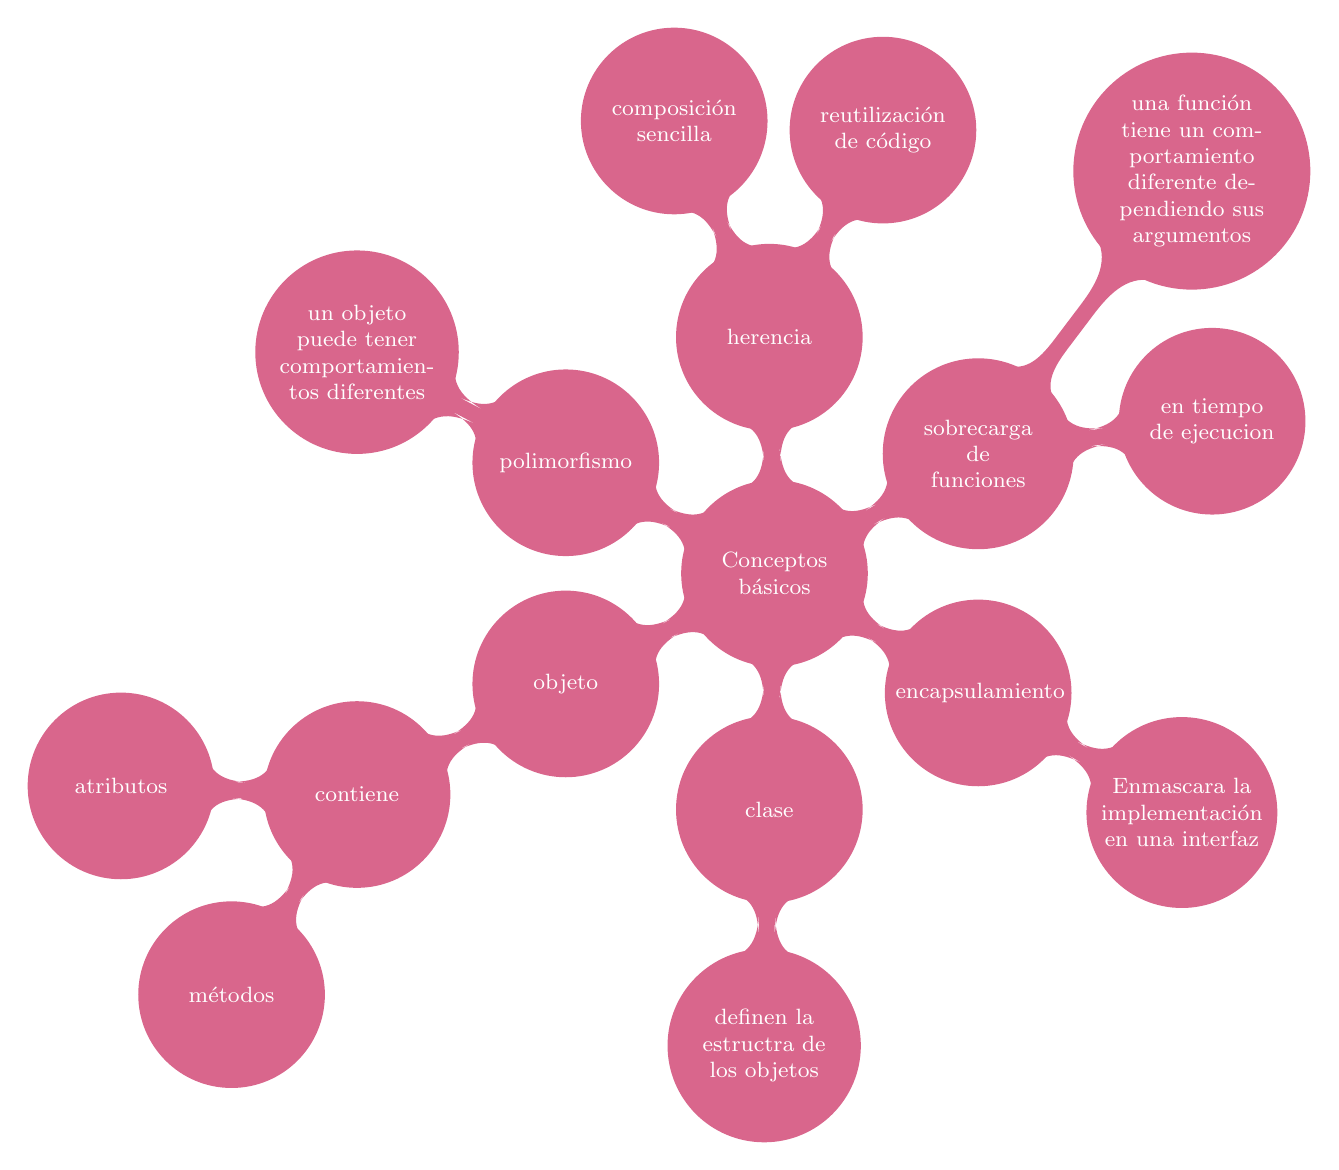
\begin{tikzpicture}[small mindmap, grow cyclic, every node/.style=concept, concept color=purple!60, text=white,
    level 1/.style={level distance=3cm,sibling angle=365/6},
    level 2/.style={level distance=3cm,sibling angle=45},
    level 3/.style={level distance=3cm,sibling angle=60}]
    \node{ Conceptos básicos }
    child { node { objeto }
        child { node { contiene }
            child { node { atributos }}
            child { node { métodos }}
        }
    }
    child { node { clase }
        child { node { definen la estructra de los objetos } }
    }
    child { node { encapsulamiento }
        child { node { Enmascara la implementación en una interfaz } }
    }
    child { node { sobrecarga\\ de\\ funciones }
        child { node { en tiempo de ejecucion } }
        child[scale=1.5] { node { una función tiene un comportamiento diferente dependiendo sus argumentos } }
    }
    child { node { herencia }
        child[sibling angle=60] { node { reutilización de código } }
        child { node { composición sencilla } }
    }
    child { node { polimorfismo }
        child { node { un objeto puede tener comportamientos diferentes } }
    }
    ;
\end{tikzpicture}
\end{center}
\end{document}
